\chapter{EXPERIMENTOS}
\label{cap-experimentos}

\section{section 00}

\blindtext

Here (Fig.~\ref{fig:multi-figures}) it goes an example of figures, captions, and references (e.g. \ref{fig:img01, fig:img02})

\begin{figure}[h!]
	\centering
  \subfloat[]{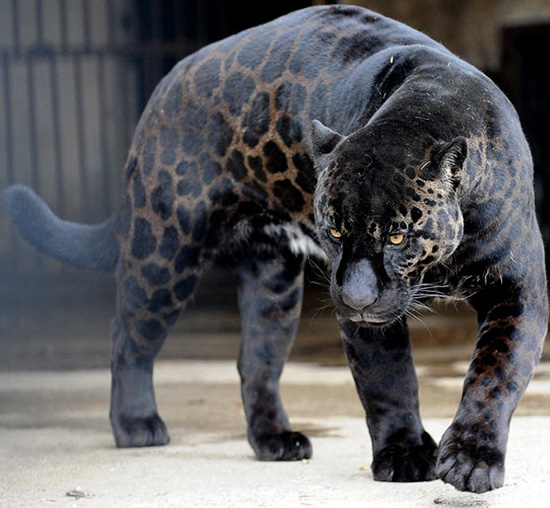
\includegraphics[width=4.5cm]{img01}\label{fig:img01}} { } \subfloat[]{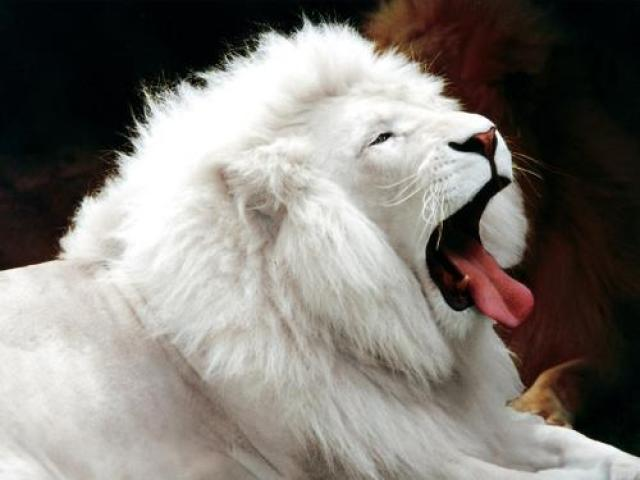
\includegraphics[width=4.5cm]{img02}\label{fig:img02}} { }
  \subfloat[]{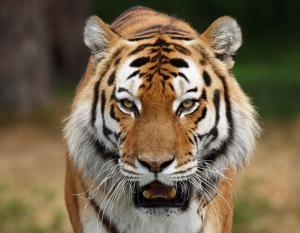
\includegraphics[width=4.5cm]{img03}\label{fig:img03}} \\
  \subfloat[]{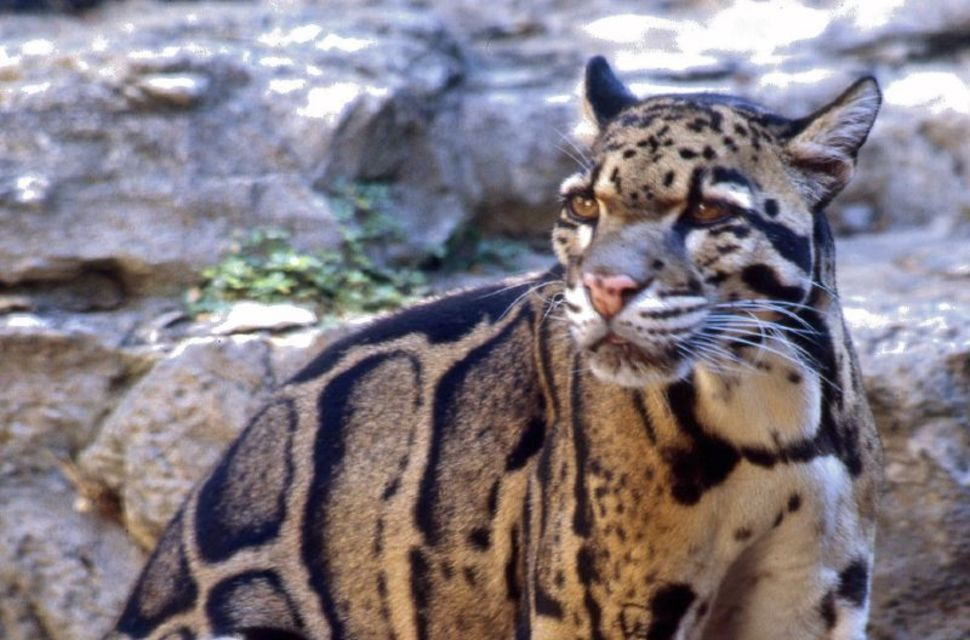
\includegraphics[width=4.5cm]{img04}\label{fig:img04}} { }
  \subfloat[]{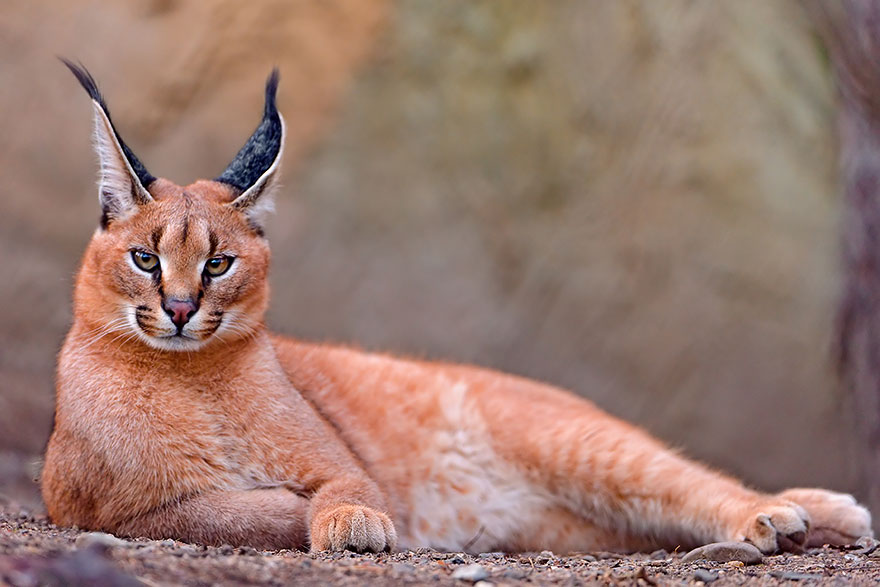
\includegraphics[width=4.5cm]{img05}\label{fig:img05}} { }
  \subfloat[]{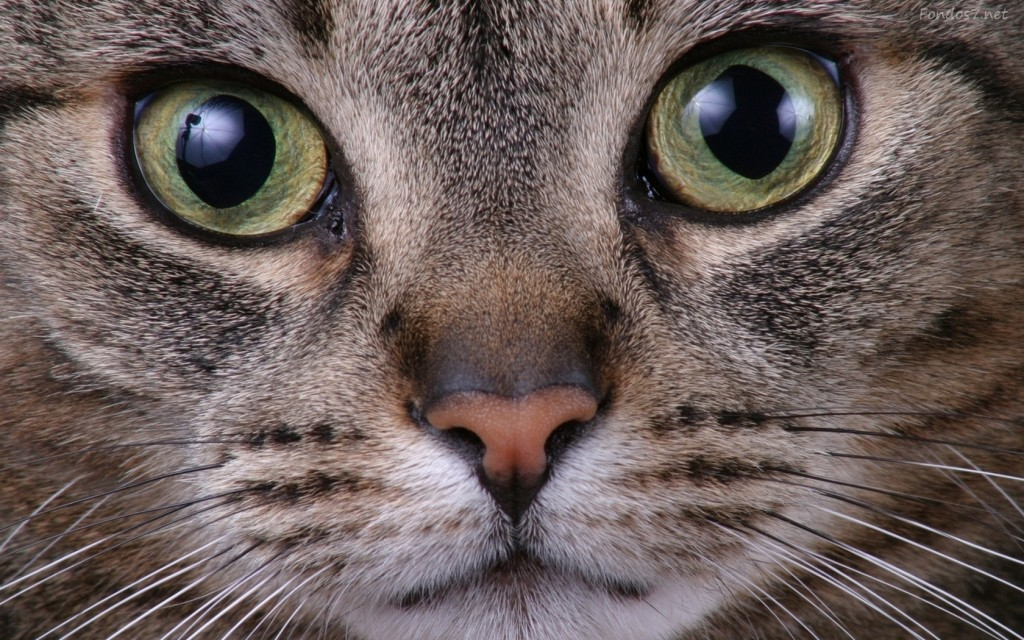
\includegraphics[width=4.5cm]{img06}\label{fig:img06}} { }
  \caption[caption short-format to be shown on list-of-figures]{caption-long-format to be shown on the page}
	\label{fig:multi-figures}
\end{figure}

\blindtext

\newcolumntype{L}[1]{>{\hsize=#1\hsize\raggedright\arraybackslash}X}%
\newcolumntype{R}[1]{>{\hsize=#1\hsize\raggedleft\arraybackslash}X}%
\newcolumntype{C}[2]{>{\hsize=#1\hsize\columncolor{#2}\centering\arraybackslash}X}%

%%TABLA COLOR FILTERING
\begin{center}
\begin{table}[H]
\begin{tabularx}{\textwidth}[t]{ L{0.7}  L{1.3} }
\hline
\textbf{\textcolor{myGreen}{\textit{Beautiful table}}} & \\
\hline
A \textit{topic 1}. & 
\begin{minipage}[t]{1.3\linewidth}%
\begin{itemize}
\item[A.1] text-a-1.
\item[A.2] text-a-2.
\item[A.3] text-a-3.

\end{itemize} 
\end{minipage}\\
\hline
B \textit{topic 2} &
\begin{minipage}[t]{1.3\linewidth}%
\begin{itemize}
\item[B.1] text-b-1.
\item[B.2] text-b-2.
\item[B.3] text-b-3.

\end{itemize} 
\end{minipage}
\end{tabularx}
\caption{This is a so-beauty table.}
\label{tab:beauty}
\end{table}
\end{center}


\blindtext
